\documentclass[main.tex]{subfiles}
\begin{document}

\section{Implement a C bytestream parsing function for a weather data sensor}
Use the header in listing \ref{code:bytestream-header}. Note that within the \texttt{weather\_data\_t} structure, the temperature is stored as a float with units of degrees Celsius, while the pressure is stored as a float with units of \textbf{kilopascals}. The function will only be called on a complete packet (i.e. the entire packet is received before the function is called).

\lstinputlisting[caption={Bytestream Parsing Header}, label={code:bytestream-header}]{code/packet_parsing/packet_parsing_header.h}

\subsection{Sample Datasheet}
The weather sensor outputs a UART packet with the following format. A graphical version of the packet format is shown in figure \ref{fig:packet-data}.
\begin{table}[h!]
    \centering
    \begin{tabular}{|c|l|}
    \hline
    \textbf{Byte} & \textbf{Description} \\ \hline
    0 & Start of Frame (0x55) \\ \hline
    1 & Temperature data (Celsius) - Integer part + 32 ($T_{integer} = Byte_{1} - 32$)  \\ \hline
    2 & Temperature data (Celsius) - Fractional part \\ \hline
    3 & Pressure data (Pa - Integer Part) - MSB \\ \hline
    4 & Pressure data (Pa - Integer Part) \\ \hline
    5 & Pressure data (Pa - Integer Part) \\ \hline
    6 & Pressure data (Pa - Integer Part) - LSB \\ \hline
    7 & Checksum - Lowest byte of the sum of bytes 1-6 \\ \hline
    \end{tabular}
    \caption{Byte Descriptions for Weather Sensor UART Packet}
    \label{table:byte_description}
\end{table}
    

\begin{figure}[H]
    \centering
    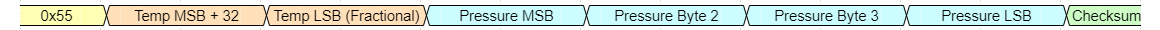
\includegraphics[width=1.0\textwidth]{generated_images/svg_generated/packet_parsing.png}
    \caption{Weather Sensor Packet Format}
    \label{fig:packet-data}
\end{figure}

\spoilerline

\subsection{Packet Parsing Algorithm}
A packet parsing algorithm is a staple of embedded systems programming. Generally, an implementation of such an algorithm involves receiving a buffer (packet) of bytes (also referred to as a \textit{bytestream}), followed by iterating through the buffer and extracting relevant data. If present in the packet, a checksum is used to verify the integrity of the data.

\subsubsection{Checksum}
A checksum is a simple error-detection method\footnote{In real-world implementations, a more robust method, like a cyclic redundancy check (CRC) is usually used.} that involves summing the bytes of a packet and comparing the result to a predefined value. If the checksum is incorrect, the packet is considered corrupt. In this case, the checksum is the sum of bytes 1-6. A simple algorithm for checksum calculation is shown in listing \ref{code:checksum_ex}.

\lstinputlisting[caption={Checksum Calculation Example}, label={code:checksum_ex}]{code/packet_parsing/checksum_ex.c}

\noindent For this example, the checksum is calculated by summing the bytes from 1 to 6. However, the checksum that is transmitted is the lowest byte of the sum. This is done to save bandwidth and reduce the number of bytes transmitted. It is equivalent to saying that \texttt{checksum\_transmitted = checksum\_calculated \& 0xFF}.

\subsection{Parsing Function Implementation}
When implementing a parsing function, it's important to consider the failure cases that require attention in our implementation (and usually make up most of what interviewers are expecting). In the scope of this question, the edge cases include:
\begin{itemize}
    \item The packet length is incorrect (the length is fixed and the packet is assumed to be completely received, therefore, any buffer length that is not equal to the expected packet length is considered an error).
    \item The buffer or data packet arguments are \texttt{NULL}.
    \item The start of frame byte (0x55) is not found at the beginning of the packet.
    \item The checksum is incorrect.
\end{itemize}

\noindent A sample implementation of the parsing function is shown in listing \ref{code:packet_parsing}. Note that type-punning is explicitly not used in this implementation to avoid dealing with endianness, alignment, and platform portability issues, although it is a common practice in embedded systems programming.

\lstinputlisting[caption={Packet Parsing Function}, label={code:packet_parsing}]{code/packet_parsing/parsing_implementation.c}

\subsubsection{Testing}
In some interviews, an interviewer may ask you to write a test function to verify that the parsing function works correctly. The list of edge cases mentioned above can be used to write test cases - this is further elaborated upon in \nameref{appendix:packet_parsing_tests}.

\subsection{Follow-ups}
\begin{itemize}
    \item \textbf{How would you modify the parsing function to handle a packet with a different checksum algorithm?}
    \item \textbf{How would you modify the parsing function to handle asynchronous data transmission (i.e. fragmented packets)}?
\end{itemize}

\end{document}